% Options for packages loaded elsewhere
\PassOptionsToPackage{unicode}{hyperref}
\PassOptionsToPackage{hyphens}{url}
\PassOptionsToPackage{dvipsnames,svgnames,x11names}{xcolor}
%
\documentclass[
]{report}

\usepackage{amsmath,amssymb}
\usepackage{iftex}
\ifPDFTeX
  \usepackage[T1]{fontenc}
  \usepackage[utf8]{inputenc}
  \usepackage{textcomp} % provide euro and other symbols
\else % if luatex or xetex
  \usepackage{unicode-math}
  \defaultfontfeatures{Scale=MatchLowercase}
  \defaultfontfeatures[\rmfamily]{Ligatures=TeX,Scale=1}
\fi
\usepackage{lmodern}
\ifPDFTeX\else  
    % xetex/luatex font selection
\fi
% Use upquote if available, for straight quotes in verbatim environments
\IfFileExists{upquote.sty}{\usepackage{upquote}}{}
\IfFileExists{microtype.sty}{% use microtype if available
  \usepackage[]{microtype}
  \UseMicrotypeSet[protrusion]{basicmath} % disable protrusion for tt fonts
}{}
\makeatletter
\@ifundefined{KOMAClassName}{% if non-KOMA class
  \IfFileExists{parskip.sty}{%
    \usepackage{parskip}
  }{% else
    \setlength{\parindent}{0pt}
    \setlength{\parskip}{6pt plus 2pt minus 1pt}}
}{% if KOMA class
  \KOMAoptions{parskip=half}}
\makeatother
\usepackage{xcolor}
\usepackage[lmargin=30mm,rmargin=30mm]{geometry}
\usepackage{soul}
\setlength{\emergencystretch}{3em} % prevent overfull lines
\setcounter{secnumdepth}{-\maxdimen} % remove section numbering
% Make \paragraph and \subparagraph free-standing
\ifx\paragraph\undefined\else
  \let\oldparagraph\paragraph
  \renewcommand{\paragraph}[1]{\oldparagraph{#1}\mbox{}}
\fi
\ifx\subparagraph\undefined\else
  \let\oldsubparagraph\subparagraph
  \renewcommand{\subparagraph}[1]{\oldsubparagraph{#1}\mbox{}}
\fi


\providecommand{\tightlist}{%
  \setlength{\itemsep}{0pt}\setlength{\parskip}{0pt}}\usepackage{longtable,booktabs,array}
\usepackage{calc} % for calculating minipage widths
% Correct order of tables after \paragraph or \subparagraph
\usepackage{etoolbox}
\makeatletter
\patchcmd\longtable{\par}{\if@noskipsec\mbox{}\fi\par}{}{}
\makeatother
% Allow footnotes in longtable head/foot
\IfFileExists{footnotehyper.sty}{\usepackage{footnotehyper}}{\usepackage{footnote}}
\makesavenoteenv{longtable}
\usepackage{graphicx}
\makeatletter
\def\maxwidth{\ifdim\Gin@nat@width>\linewidth\linewidth\else\Gin@nat@width\fi}
\def\maxheight{\ifdim\Gin@nat@height>\textheight\textheight\else\Gin@nat@height\fi}
\makeatother
% Scale images if necessary, so that they will not overflow the page
% margins by default, and it is still possible to overwrite the defaults
% using explicit options in \includegraphics[width, height, ...]{}
\setkeys{Gin}{width=\maxwidth,height=\maxheight,keepaspectratio}
% Set default figure placement to htbp
\makeatletter
\def\fps@figure{htbp}
\makeatother

\makeatletter
\makeatother
\makeatletter
\makeatother
\makeatletter
\@ifpackageloaded{caption}{}{\usepackage{caption}}
\AtBeginDocument{%
\ifdefined\contentsname
  \renewcommand*\contentsname{Table of contents}
\else
  \newcommand\contentsname{Table of contents}
\fi
\ifdefined\listfigurename
  \renewcommand*\listfigurename{List of Figures}
\else
  \newcommand\listfigurename{List of Figures}
\fi
\ifdefined\listtablename
  \renewcommand*\listtablename{List of Tables}
\else
  \newcommand\listtablename{List of Tables}
\fi
\ifdefined\figurename
  \renewcommand*\figurename{Figure}
\else
  \newcommand\figurename{Figure}
\fi
\ifdefined\tablename
  \renewcommand*\tablename{Table}
\else
  \newcommand\tablename{Table}
\fi
}
\@ifpackageloaded{float}{}{\usepackage{float}}
\floatstyle{ruled}
\@ifundefined{c@chapter}{\newfloat{codelisting}{h}{lop}}{\newfloat{codelisting}{h}{lop}[chapter]}
\floatname{codelisting}{Listing}
\newcommand*\listoflistings{\listof{codelisting}{List of Listings}}
\makeatother
\makeatletter
\@ifpackageloaded{caption}{}{\usepackage{caption}}
\@ifpackageloaded{subcaption}{}{\usepackage{subcaption}}
\makeatother
\makeatletter
\@ifpackageloaded{tcolorbox}{}{\usepackage[skins,breakable]{tcolorbox}}
\makeatother
\makeatletter
\@ifundefined{shadecolor}{\definecolor{shadecolor}{rgb}{.97, .97, .97}}
\makeatother
\makeatletter
\makeatother
\makeatletter
\makeatother
\makeatletter
\@ifpackageloaded{fontawesome5}{}{\usepackage{fontawesome5}}
\makeatother
\ifLuaTeX
  \usepackage{selnolig}  % disable illegal ligatures
\fi
\IfFileExists{bookmark.sty}{\usepackage{bookmark}}{\usepackage{hyperref}}
\IfFileExists{xurl.sty}{\usepackage{xurl}}{} % add URL line breaks if available
\urlstyle{same} % disable monospaced font for URLs
\hypersetup{
  colorlinks=true,
  linkcolor={blue},
  filecolor={Maroon},
  citecolor={Blue},
  urlcolor={Blue},
  pdfcreator={LaTeX via pandoc}}

\author{}
\date{}

\begin{document}
\ifdefined\Shaded\renewenvironment{Shaded}{\begin{tcolorbox}[boxrule=0pt, sharp corners, borderline west={3pt}{0pt}{shadecolor}, enhanced, frame hidden, breakable, interior hidden]}{\end{tcolorbox}}\fi

\hypertarget{profile-pic}{}
\begin{figure}

{\centering 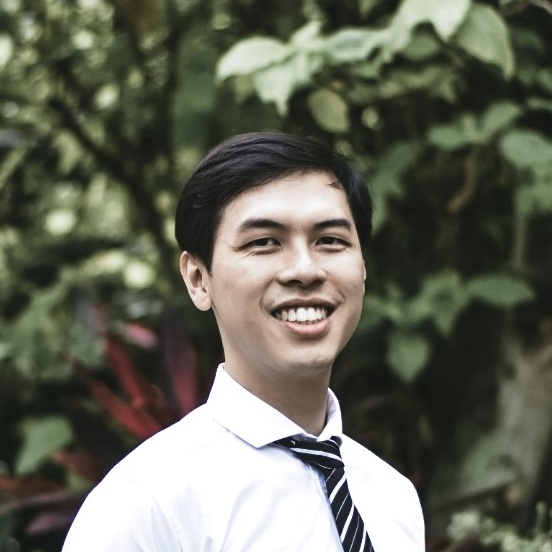
\includegraphics[width=2.08333in,height=\textheight]{images/profile.jpg}

}

\end{figure}

\hypertarget{lam-bhan}{%
\section{\texorpdfstring{\ul{Lam} Bhan}{Lam Bhan}}\label{lam-bhan}}

BEng, PhD \faIcon{briefcase} Research Assistant Professor
\faIcon{building-columns} Nanyang Technological University

\href{https://scholar.google.com.sg/citations?user=22NFnNsAAAAJ\&hl=en}{}~~
\href{https://orcid.org/0000-0001-5193-6560}{}~~
\href{https://www.webofscience.com/wos/author/record/O-2911-2013}{}~~
\href{https://www.researchgate.net/profile/Bhan-Lam}{}~~
\href{https://github.com/bhanlam}{\faIcon{github-square}}~~
\href{https://twitter.com/bhanlam}{\faIcon{twitter-square}}~~
\href{https://www.linkedin.com/in/lambhan/}{\faIcon{linkedin}}~~
\href{mailto:bhanlam@ntu.edu.sg}{\faIcon{envelope-square}}

\hypertarget{fa-hand-point-up-about-me}{%
\subsection{\texorpdfstring{\faIcon{hand-point-up} About
Me}{ About Me}}\label{fa-hand-point-up-about-me}}

\begin{quote}
Intrigued about all things sound \faIcon{volume-high} Currently engaged
in soundscape research and developing active noise control systems for
the betterment of urban liveability and sustainability
\faIcon{tree-city}.
\end{quote}

Check out my full CV here: \href{./cv/index.qmd}{\faIcon{address-card}
CV} All my Publications here:
\href{./publications/index.qmd}{\faIcon{file-lines} Publications}

\faIcon{bullhorn} \textbf{Call for papers!}

\includegraphics[width=2.60417in,height=\textheight]{images/CALL FOR PAPERS.png}

\faIcon{calendar-days} \textbf{Upcoming event:}
\href{https://internoise2023.org/}{
\includegraphics[width=2.60417in,height=\textheight]{index_files/mediabag/images/logo-in2023.pdf}}

\hypertarget{fa-file-lines-a-summary-of-publication-citation-metrics}{%
\subsection{\texorpdfstring{\faIcon{file-lines} A Summary of Publication
\& Citation
metrics}{ A Summary of Publication \& Citation metrics}}\label{fa-file-lines-a-summary-of-publication-citation-metrics}}

\hypertarget{citation-trend-google-scholar}{%
\subsubsection{Citation Trend (Google
Scholar)}\label{citation-trend-google-scholar}}

\begin{figure}

{\centering 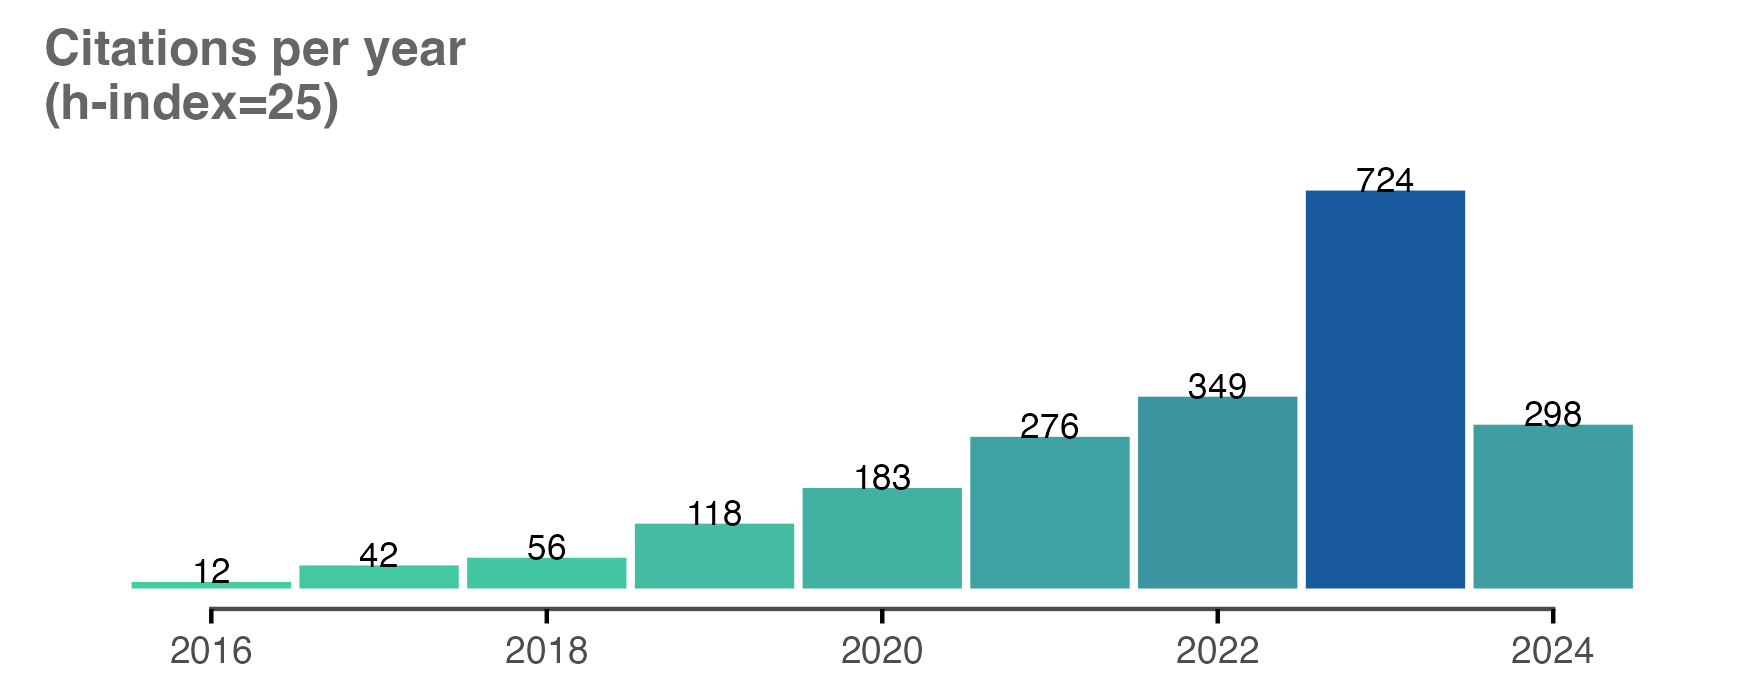
\includegraphics{images/citeHistory.png}

}

\end{figure}

\hypertarget{citation-pic}{}
\hypertarget{citation-breakdown-per-article-google-scholar}{%
\subsubsection{Citation breakdown per article (Google
Scholar)}\label{citation-breakdown-per-article-google-scholar}}

\begin{figure}

{\centering 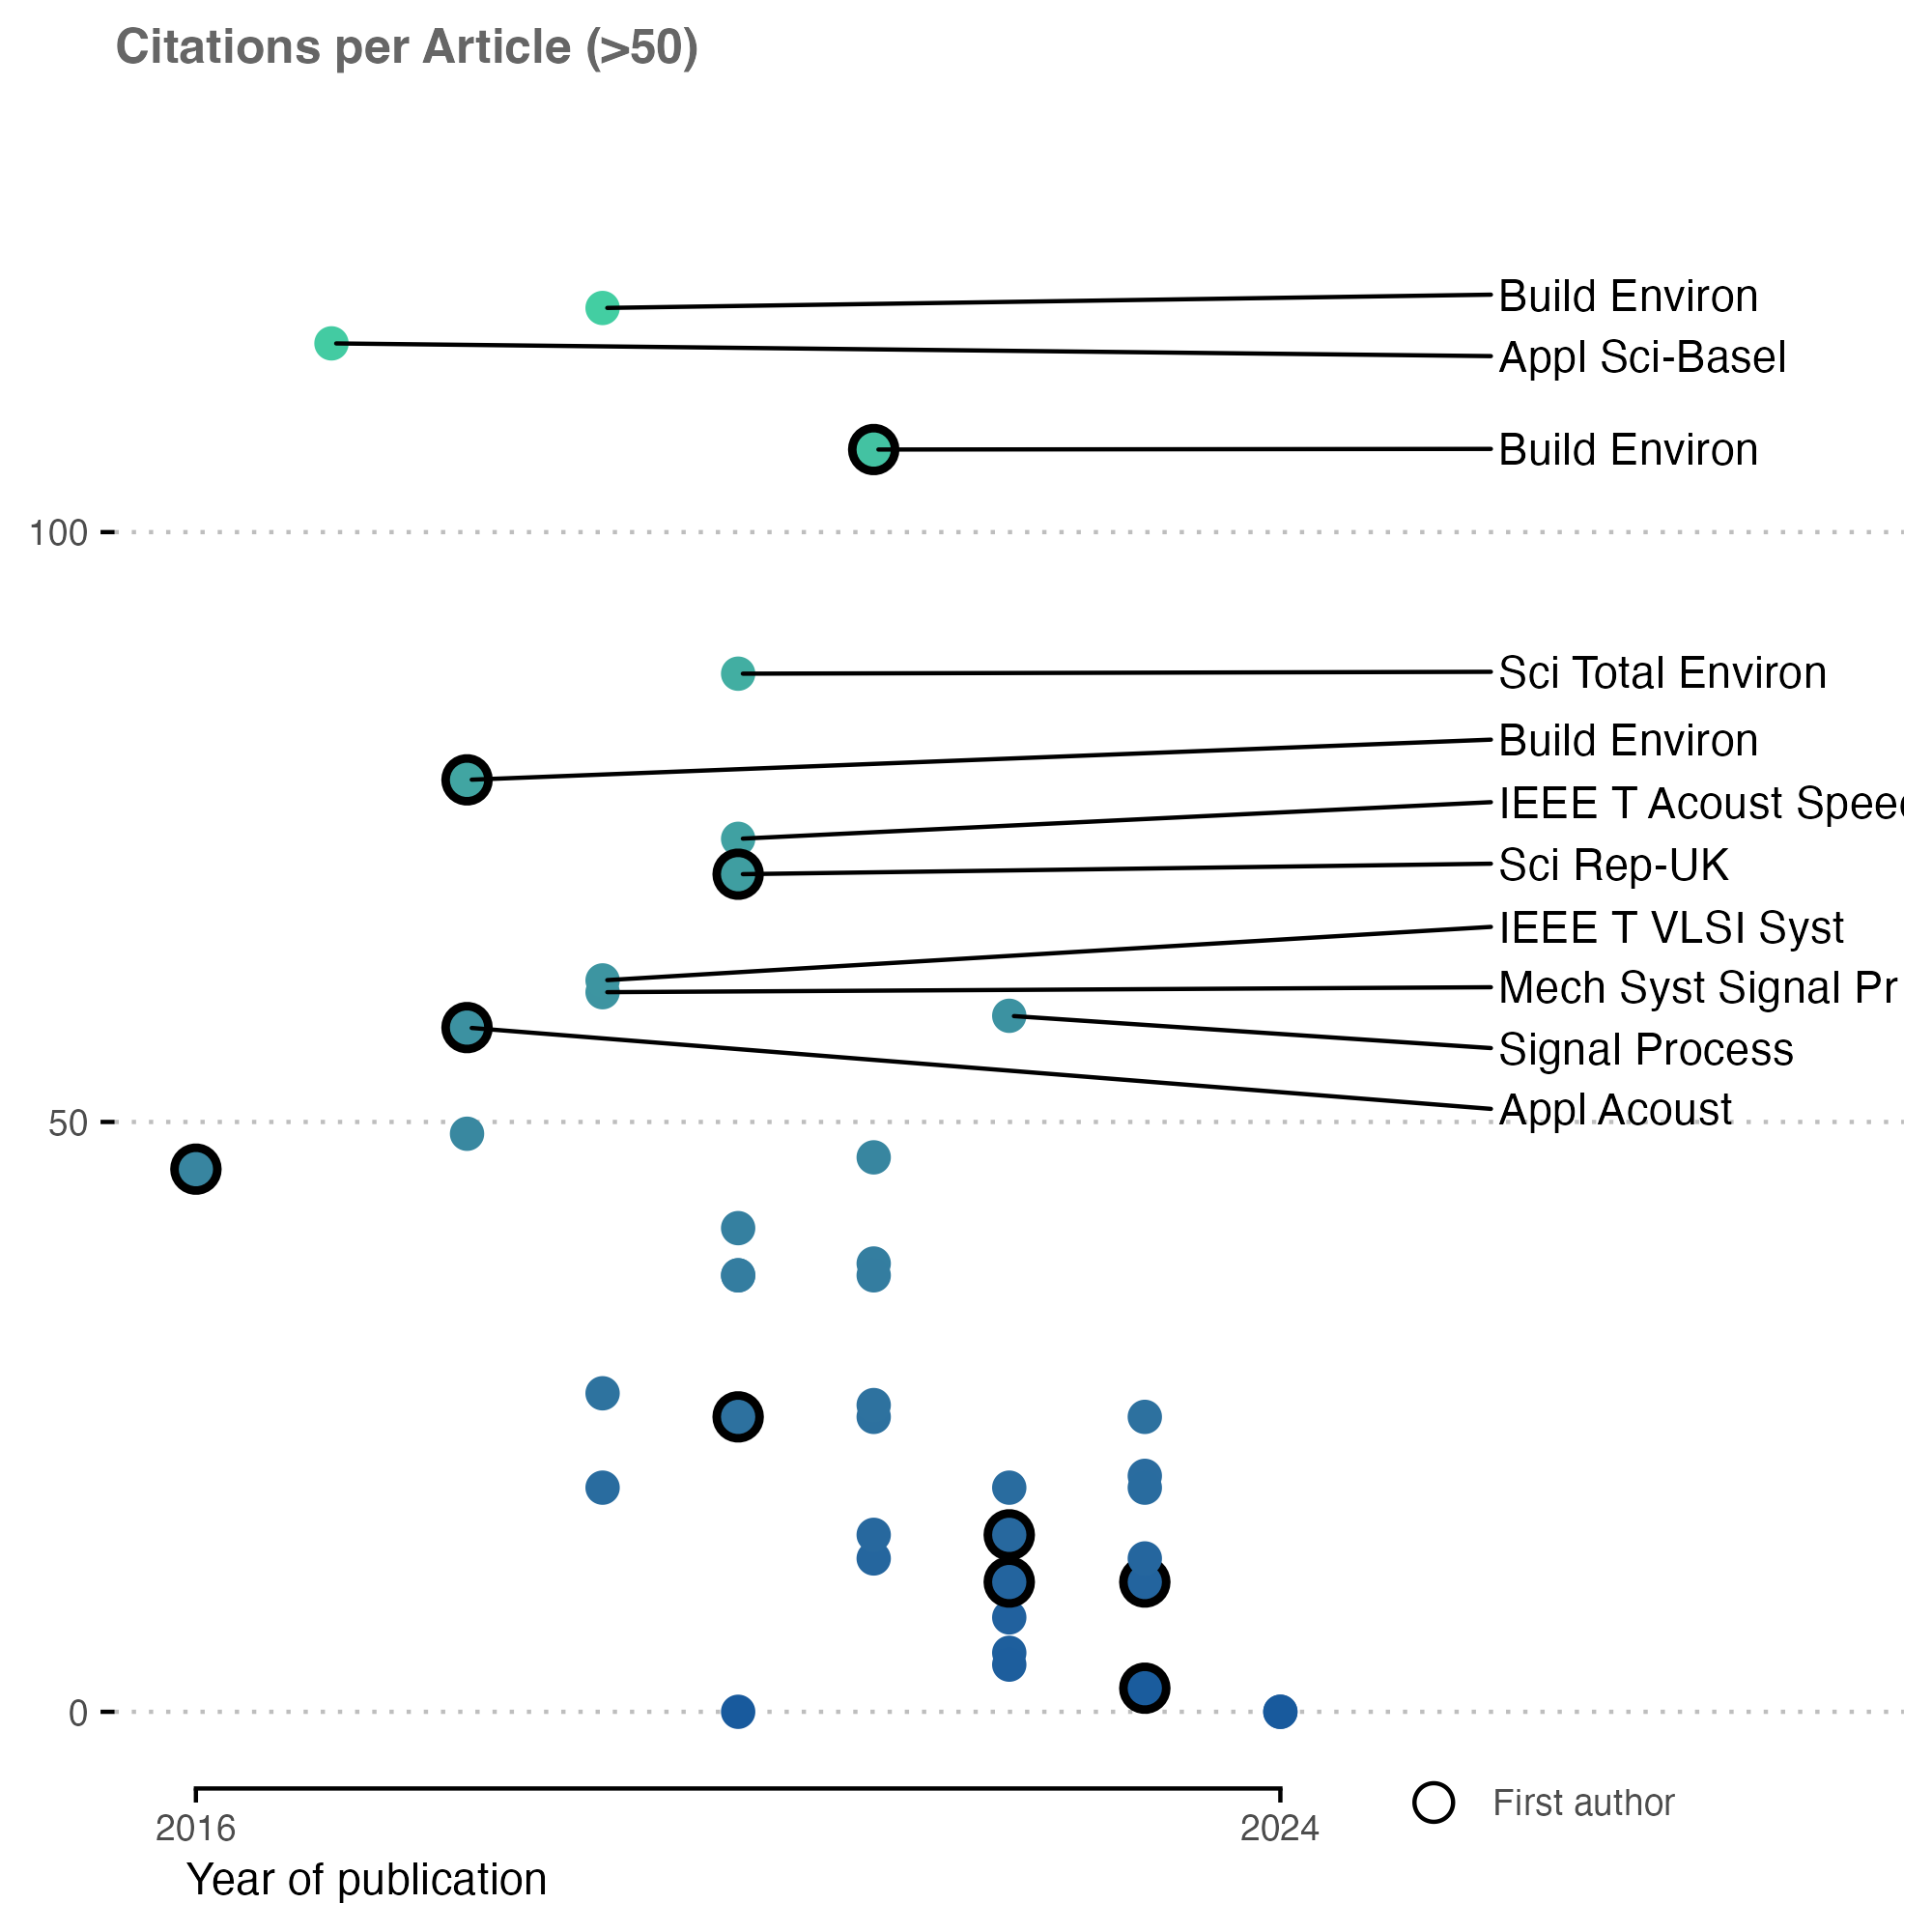
\includegraphics{images/citationsPerArticle.png}

}

\end{figure}

\hypertarget{citation-pic}{}
\hypertarget{journal-impact-factor-trend}{%
\subsubsection{Journal Impact Factor
Trend}\label{journal-impact-factor-trend}}

\begin{figure}

{\centering 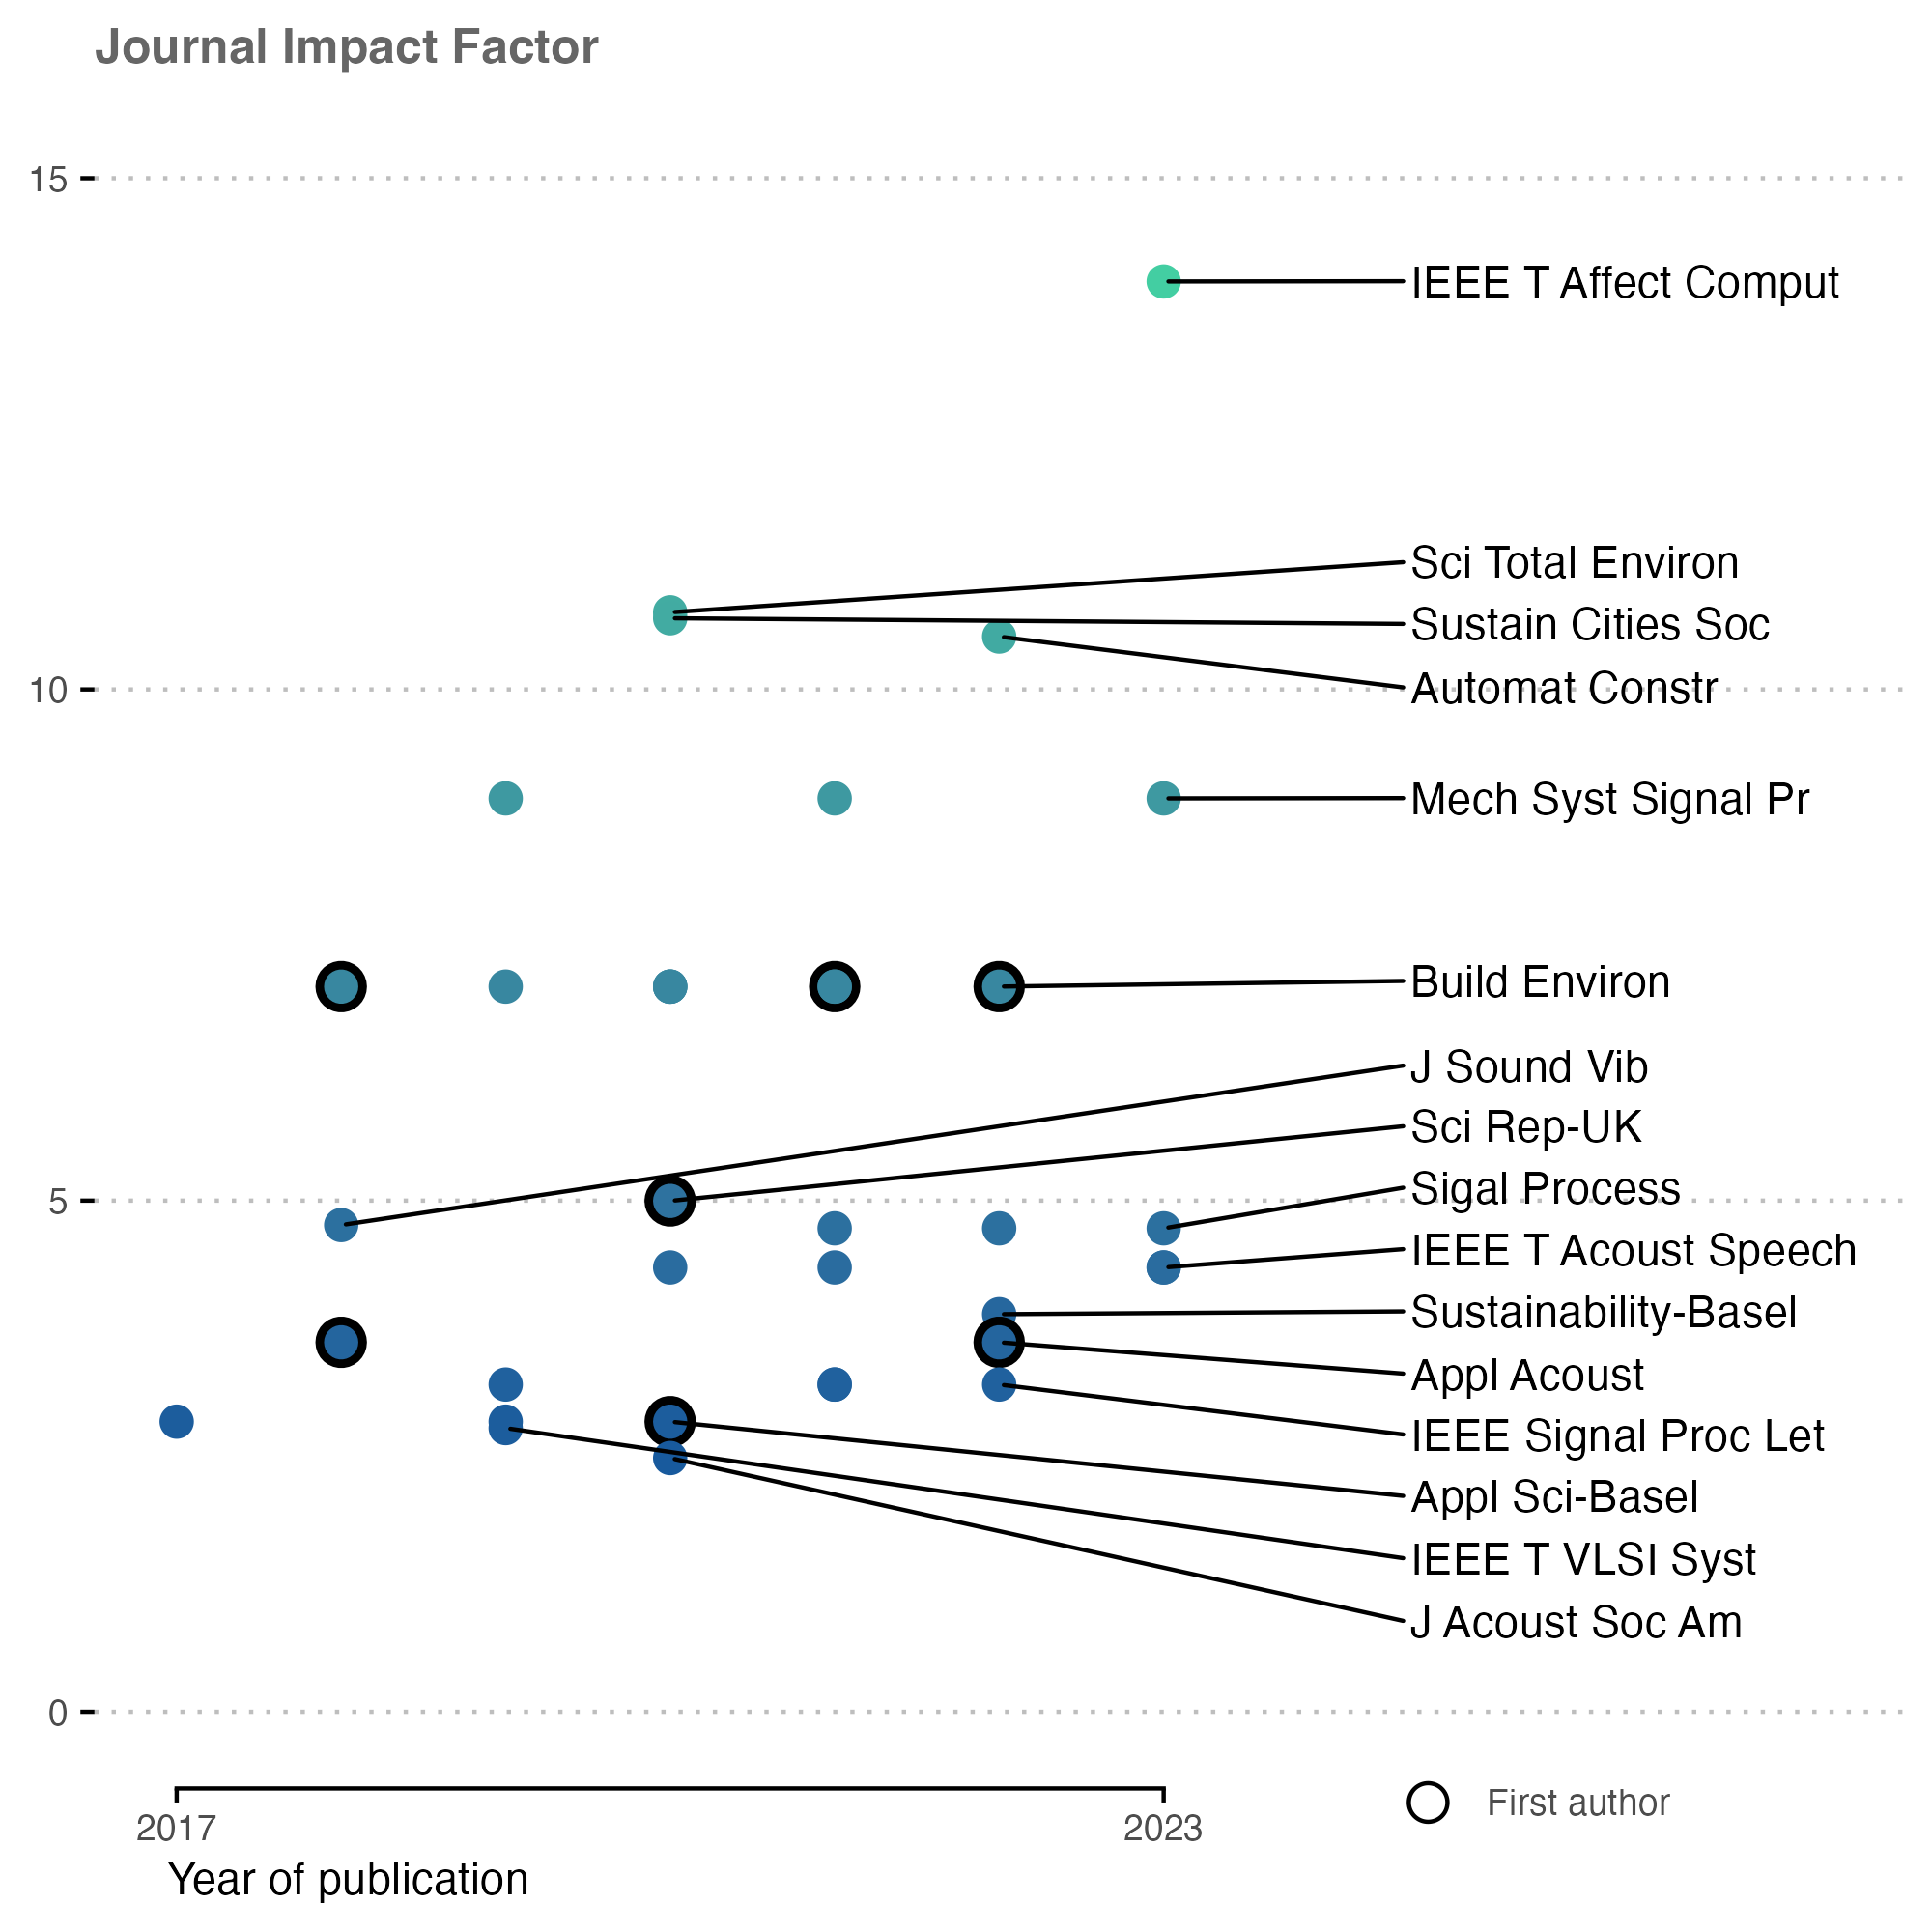
\includegraphics{images/journalIF.png}

}

\end{figure}



\end{document}
